% ============================================================
%  chapter02c_statistical_inference_slides.tex
%  Chapter 2: Background -- Section 2.3
%  Statistical Inference and Estimation
%  An Introduction to Universal Artificial Intelligence
%  Marcus Hutter, Elliot Catt & David Quarel -- CRC Press, 2024
% ============================================================
\documentclass[aspectratio=169,10pt]{beamer}

\usetheme{Madrid}
\usecolortheme{seahorse}
\usefonttheme{professionalfonts}

% -- packages ------------------------------------------------------------------
\usepackage{amsmath,amssymb,bm}
\usepackage{graphicx}
\usepackage{booktabs}
\usepackage{listings}
\usepackage{xcolor}
\usepackage{tikz}
\usetikzlibrary{shapes,arrows,positioning,calc}
\usepackage{mathtools}
\usepackage{array}
\usepackage{multirow}

\graphicspath{{figures/}}

% -- listings style --------------------------------------------------------
\lstdefinestyle{pythonstyle}{
  language=Python,
  basicstyle=\ttfamily\scriptsize,
  keywordstyle=\color{blue}\bfseries,
  stringstyle=\color{orange},
  commentstyle=\color{green!50!black}\itshape,
  numberstyle=\tiny\color{gray},
  numbers=left,
  stepnumber=1,
  numbersep=5pt,
  frame=single,
  backgroundcolor=\color{gray!7},
  breaklines=true,
  showstringspaces=false,
  tabsize=2,
  captionpos=b,
}
\lstset{style=pythonstyle}

% -- beamer setup -----------------------------------------------------------
\setbeamertemplate{footline}[frame number]
\setbeamertemplate{navigation symbols}{}
\setbeamersize{text margin left=0.5cm, text margin right=0.5cm}

% -- title -------------------------------------------------------------------
\title[UAI -- Ch.2.3]{An Introduction to Universal Artificial Intelligence}
\subtitle{Chapter 2, Section 2.3: Statistical Inference and Estimation}
\author{Based on Hutter, Catt \& Quarel}
\institute{CRC Press, 2024}
\date{}

% =============================================================================
\begin{document}
% =============================================================================

\begin{frame}
  \titlepage
\end{frame}

\begin{frame}{Outline}
  \tableofcontents
\end{frame}

% =============================================================================
\section{2.3.0 Setting the Scene}
% =============================================================================

\begin{frame}[allowframebreaks]{Why Statistical Inference?}
  \textbf{The prediction problem.} Throughout this book we want an agent to
  predict what comes next in a sequence, given what it has seen so far. To make
  any progress, we first assume we know \emph{something} about the process that
  generates the sequence, and we begin with the simplest possible assumption.

  \begin{block}{The i.i.d.\ Bernoulli assumption}
    A binary sequence $x_1,x_2,\dots$ is generated \emph{independently and
    identically distributed} (i.i.d.) by a Bernoulli distribution with an
    \emph{unknown} parameter $\theta$ (theta) that must be inferred from past
    observations.
  \end{block}
  \textbf{Plain English.} ``i.i.d.'' means every symbol in the sequence is
  produced by the same random mechanism, and knowing some symbols tells you
  nothing extra about the others. $\theta \in [0,1]$ is the unknown probability
  that any given symbol equals $1$.

  \framebreak

  This assumption is strong: it says nothing depends on anything before it,
  which is often unrealistic. Later chapters relax it:
  \begin{itemize}
    \item \textbf{Chapter 3} allows the distribution to depend on \emph{any}
      past elements (general sequence prediction / induction).
    \item \textbf{Chapter 4} covers efficient predictors for sequences where
      the next symbol depends only on a \emph{bounded} number of past
      elements (finite-memory / Markov models).
  \end{itemize}

  We will study the estimation problem from two angles:
  \begin{itemize}
    \item the \textbf{frequentist} perspective (this deck), which treats
      $\theta$ as a fixed but unknown constant and studies estimators as
      functions of random data;
    \item the \textbf{Bayesian} perspective (next chapter), which treats
      $\theta$ itself as a random variable with a prior distribution that
      gets updated by evidence.
  \end{itemize}

  \textbf{Parametric models.} We assume the population/process can be fully
  described by a probability model with parameters $\theta$ drawn from a set
  $\Theta$ (Theta), often $\Theta \subseteq \mathbb{R}^d$. Inference then
  reduces to \emph{searching for the correct $\theta \in \Theta$}. For our
  running example, the Bernoulli model $\mathrm{Bern}(x;\theta)$ has
  $\Theta = [0,1] \subset \mathbb{R}$.

  For now we only want a single numerical best guess for $\theta$ given data
  $x_{1:n}$ (meaning the observations $x_1,\dots,x_n$). Later we will also
  want a measure of \emph{confidence} in that guess, e.g.\ a statement like
  $\mathbb{P}(\theta \in [0.4,0.6] \mid \mathcal{D}) $ (the probability that
  $\theta$ lies in an interval, given data $\mathcal{D}$), which requires
  interval estimation.
\end{frame}

% =============================================================================
\section{2.3.1 The Sunrise Problem}
% =============================================================================

\begin{frame}[allowframebreaks]{Example 2.3.1: The Sunrise Problem}
  \textbf{Question.} How likely is it that the sun will \emph{not} rise
  tomorrow? Consider the naive frequentist estimate
  \[
    \frac{\text{days the sun did not rise}}{\text{days the Earth (or humans) have experienced}}.
  \]
  \textbf{Plain English.} This just counts failures over total observed days.

  Since the sun has never failed to rise on any recorded day, this ratio
  gives probability $0$. But probability $0$ means ``impossible'' -- and
  declaring the event impossible, just because it has never happened yet,
  seems absurd. Solving this puzzle motivates the \emph{Laplace rule} and
  many other estimation methods used throughout the book.

  \framebreak

  \textbf{Formal setup.}
  \begin{enumerate}
    \item Sample space $\Omega = \{\text{not rise}, \text{rise}\}^n$. Define
      i.i.d.\ $\{0,1\}$-valued random variables $X_1,\dots,X_n \sim
      \mathrm{Bernoulli}(\theta)$, with fixed but unknown $\theta$. The
      variable $X_t$ returns $1$ iff the sun rose on day $t$:
      $\mathbb{P}(X_i=1)=\theta$ and $\mathbb{P}(X_i=0)=1-\theta$.
    \item We observe values $x_{1:n}$ from the $n$ i.i.d.\ random variables
      $X_1,\dots,X_n$.
    \item We wish to \emph{estimate} $\theta$ using an estimator
      $t(x_{1:n})$ -- a function of the observed data. This value is the
      outcome of the random variable $T_n(X_1,\dots,X_n)$.
    \item Based on the estimate of $\theta$, we predict $x_{n+1}$: will the
      sun rise on the next day or not?
  \end{enumerate}

  \framebreak

  \textbf{Why model the sun as i.i.d.\ Bernoulli at all?} Historically (the
  problem is 18th-century, due to Laplace), the physical mechanism behind
  sunrise was not understood. Imagine explaining this to someone who has
  never seen the sky, and only knows that each ``day'' something called the
  sun either ``rises'' or does not. With no other information, i.i.d.\ and
  Bernoulli are not unreasonable modeling choices.

  A more modern treatment would use domain knowledge from astrophysics: the
  sun is expected to keep rising for roughly the next $5$ billion years,
  until it swells up and engulfs the Earth (assuming nothing else happens
  first). We will return to this example once we have built up the tools
  (the Laplace/KT estimator) to resolve the ``probability zero'' absurdity.
\end{frame}

% =============================================================================
\section{2.3.2 Maximum Likelihood}
% =============================================================================

\begin{frame}[allowframebreaks]{The Likelihood Function}
  \textbf{Idea.} Perhaps the most important and intuitively appealing
  estimation procedure is \emph{maximum likelihood}: pick the parameter
  value that makes the data we actually observed as probable as possible.

  \begin{block}{Likelihood function}
    For a parameter $\theta$ based on a sample of $n$ random variables
    $X_1,\dots,X_n$, the \emph{likelihood function} is the joint probability
    density of the sample, viewed as a function of $\theta$:
    \[
      L(\theta) \;=\; L(\theta;x_1,\dots,x_n) \;:=\; p_{X_1,\dots,X_n}(x_1,\dots,x_n;\theta).
    \]
  \end{block}
  \textbf{Plain English.} $L(\theta)$ answers: ``if the true parameter were
  $\theta$, how likely would this exact data sample have been?'' It is a
  function of $\theta$ with the data $x_1,\dots,x_n$ held fixed.

  \framebreak

  If the $X_i$ are i.i.d.\ with pdf $p_X(x;\theta)$, the likelihood
  factorizes into a product:
  \[
    L(\theta) \;=\; \prod_{i=1}^{n} p_X(x_i;\theta).
  \]
  \textbf{Plain English.} $\prod_{i=1}^n$ (product from $i=1$ to $n$) just
  multiplies the individual densities $p_X(x_i;\theta)$ together, one per
  data point -- valid because independence lets probabilities of separate
  events multiply.

  $L(\theta)$ can be thought of as the joint conditional probability
  $p(x_1,\dots,x_n \mid \theta)$. For this factorization to hold we need the
  $X_i$ to be \emph{conditionally} i.i.d.\ given $\theta$:
  \[
    \mathbb{P}(x_1,\dots,x_n \mid \theta) \;=\; \prod_{i=1}^n p(x_i \mid \theta).
  \]

  \framebreak

  \begin{block}{Maximum likelihood estimator (MLE)}
    The MLE of $\theta$ is the value that maximizes the likelihood:
    \[
      \widehat{\theta}_{ML} \;:=\; \operatorname*{arg\,sup}_{\theta \in \Theta} L(\theta;x_1,\dots,x_n).
    \]
  \end{block}
  \textbf{Plain English.} $\operatorname*{arg\,sup}_{\theta \in \Theta}$
  (``argument of the supremum'') means: search over every allowed parameter
  value $\theta$ in $\Theta$ and return the one that makes $L(\theta)$
  largest.

  In practice we use the \emph{log-likelihood} $\ln L(\theta)$, since $\ln$
  is monotonically increasing (so maximizing $L$ or $\ln L$ gives the same
  $\theta$), and logs turn products into sums, which are far easier to
  differentiate:
  \[
    \operatorname*{arg\,sup}_{\theta \in \Theta} L(\theta)
    \;=\; \operatorname*{arg\,sup}_{\theta \in \Theta} \ln L(\theta),
    \qquad
    \ln L(\theta) \;=\; \ln\!\Big(\prod_{i=1}^n p_X(x_i;\theta)\Big) \;=\; \sum_{i=1}^n \ln p_X(x_i;\theta).
  \]
  The derivative $\nabla_\theta \ln L(\theta)$ (gradient with respect to
  $\theta$) is easier to compute than $\nabla_\theta L(\theta)$ because
  derivatives are linear operators, and setting it to zero locates the
  maximizing $\theta$.
\end{frame}

\begin{frame}[allowframebreaks]{Example 2.3.2: MLE of a Bernoulli Sequence}
  Suppose $X_1,\dots,X_n \sim \mathrm{Bern}(x;\theta)$ with unknown
  $\theta$, where
  \[
    \mathrm{Bern}(x;\theta) \;=\; \theta^x (1-\theta)^{1-x}.
  \]
  \textbf{Plain English.} This single formula gives $\theta$ when $x=1$ and
  $1-\theta$ when $x=0$ -- exactly the two Bernoulli outcomes, written
  compactly using exponents.

  The log-likelihood is
  \[
    \ln L(\theta) \;=\; \sum_{i=1}^n \big[x_i \ln\theta + (1-x_i)\ln(1-\theta)\big].
  \]

  \framebreak

  Differentiating with respect to $\theta$:
  \[
    \nabla_\theta \ln L(\theta) \;=\; \sum_{i=1}^n \left[\frac{x_i}{\theta} + \frac{x_i - 1}{1-\theta}\right].
  \]
  Setting this equal to zero and solving for $\theta$ gives the MLE:
  \[
    \boxed{\widehat{\theta}_{ML} \;=\; \frac{1}{n}\sum_{i=1}^n x_i}
  \]
  \textbf{Plain English.} The MLE of a Bernoulli parameter is simply the
  \emph{sample average} -- the fraction of $1$'s observed. This matches
  intuition: since $\mathbb{E}[X]=\theta$ for $X \sim \mathrm{Bern}(\theta)$,
  averaging samples estimates the expectation, which equals $\theta$.

  We call estimators of this ``proportion of $1$'s'' form \emph{frequency
  estimators}.

  \framebreak

  \textbf{Back to the sunrise problem.} The MLE gives $\widehat{\theta}_{ML}
  = 1$ whenever every observed day the sun rose (no zeros at all in the
  data). This implies the sun will rise tomorrow with \emph{absolute
  certainty} -- again the nonsensical, overconfident answer.

  More formally: if $\mathbb{P}(A)=1$, then for any event $B$ with
  $\mathbb{P}(B)>0$,
  \[
    \mathbb{P}(A\mid B) = \mathbb{P}(A \cap B)/\mathbb{P}(B) = 1.
  \]
  \textbf{Plain English.} Once you assign probability $1$ to an event, no
  future evidence $B$ can ever change that probability -- the posterior is
  ``stuck''. This is an undesirable property for an estimator: it should
  stay open to revision.
\end{frame}

% =============================================================================
\section{2.3.3 Reparametrization Equivariance}
% =============================================================================

\begin{frame}{Reparametrization Equivariance of the MLE}
  We parameterized the Bernoulli model by $\theta$, the probability of
  observing a $1$. But we could equally have chosen a different
  parametrization -- e.g.\ the probability of observing a $0$, or the
  \emph{square} of the probability of observing a $1$. In general we can
  reparameterize via $\tau = \psi(\theta)$ (tau equals psi of theta) for any
  bijection $\psi$ (psi). We would expect the MLE to be \emph{invariant}
  under this change: $\widehat{\tau}_{ML} = \psi(\widehat{\theta}_{ML})$.

  \begin{block}{Proposition 2.3.3 (Reparametrization equivariance of the MLE)}
    Let $x_1,\dots,x_n$ be i.i.d.\ samples with likelihood function
    $L(\theta;x_1,\dots,x_n)$, and let $\widehat{\theta}_{ML}$ be the MLE of
    $\theta$. For any bijective function $\tau$, define the induced
    likelihood
    \[
      \tilde{L}(\tau(\theta);x_1,\dots,x_n) \;:=\; L(\theta;x_1,\dots,x_n),
    \]
    and let $\widehat{\tau}_{ML}$ maximize $\tilde{L}$. Then
    \[
      \widehat{\tau}_{ML} \;=\; \tau(\widehat{\theta}_{ML}).
    \]
  \end{block}
  \textbf{Plain English.} It does not matter whether you first find the MLE
  of $\theta$ and then transform it, or directly maximize likelihood in the
  new parametrization $\tau$ -- you land on the same answer. Relabeling
  parameters cannot change what the ``most likely'' explanation of the data
  is.
\end{frame}

% =============================================================================
\section{2.3.4 Consistency}
% =============================================================================

\begin{frame}{Motivation: Beyond a Single Good Property}
  The MLE is intuitively appealing, but it has problems -- it depends
  wholly on the data present, which can lead to \emph{overfitting} when
  little data is available (as the sunrise problem illustrated). This
  section studies whether the MLE (and estimators in general) behave well
  \emph{asymptotically}, as the number of samples $n \to \infty$.

  For a sequence of i.i.d.\ random variables $X_1, X_2, \dots$ controlled
  by parameter $\theta$, an \emph{estimator} $T_n$ is a measurable function
  of only the first $n$ variables:
  \[
    T_n : \mathcal{X}_1 \times \dots \times \mathcal{X}_n \to \Theta,
    \qquad \text{i.e.} \quad T_n(X_1,\dots,X_n) \in \Theta,
  \]
  where $\mathcal{X}_i = X_i(\Omega)$ is the alphabet (set of possible
  outcomes) of $X_i$. Since $T_n$ is a function of random variables, $T_n$
  is itself a random variable. We study its \emph{asymptotic behavior} as
  $n \to \infty$.
\end{frame}

\begin{frame}{Definition 2.3.4: Estimator Consistency}
  \begin{block}{Definition 2.3.4 (Estimator consistency)}
    Given a sequence of i.i.d.\ random variables $(X_i)_{i=1}^\infty$ with
    distribution controlled by parameter $\theta \in \Theta$, an estimator
    $T_n$ for $\theta$ is \emph{consistent} if
    \[
      T_n \xrightarrow{P} \theta.
    \]
  \end{block}
  \textbf{Plain English.} $\xrightarrow{P}$ means \emph{convergence in
  probability}: as we gather more and more samples ($n \to \infty$), the
  estimator's value gets arbitrarily close to the true parameter $\theta$
  with probability approaching $1$. Informally: more data $\Rightarrow$
  better estimate, with (arbitrarily) high confidence.

  \textbf{Example.} The estimator $T_n = \frac{1}{n}\sum_{i=1}^n X_i$ for a
  Bernoulli $\theta$ is consistent (and in fact unbiased -- see below),
  since
  \[
    \mathbb{E}[T_n] = \theta \qquad \text{and} \qquad
    \mathbf{Var}[T_n] = \frac{\theta(1-\theta)}{n} \longrightarrow 0.
  \]
  \textbf{Plain English.} As $n$ grows, the spread (variance) of the
  estimator around its correct average value shrinks to zero, so it
  concentrates tightly on $\theta$.

  Consistency alone is a fairly \emph{weak} property: an estimator can
  still be biased -- systematically over- or under-estimating $\theta$ --
  even while converging in the limit.
\end{frame}

\begin{frame}[allowframebreaks]{Definition 2.3.5: Estimator Bias, and Two Contrasting Examples}
  \begin{block}{Definition 2.3.5 (Estimator bias)}
    Given $(X_i)_{i=1}^\infty$ as above, the \emph{bias} of an estimator
    $T_n$ is
    \[
      \mathrm{Bias}(T_n) \;:=\; \mathbb{E}_\theta[T_n] - \theta.
    \]
    If $\mathrm{Bias}(T_n)=0$ for all $n\geq 1$ and all $\theta \in \Theta$,
    then $T_n$ is called \emph{unbiased}. Here $\mathbb{E}_\theta[T_n]$
    means the expectation taken with respect to the pdf $p_X(\cdot;\theta)$.
  \end{block}
  \textbf{Plain English.} Bias measures how far the estimator's
  \emph{average} value (over many hypothetical repetitions of the
  experiment) is from the true $\theta$. Zero bias means it is correct on
  average, even though any single estimate may be off.

  \framebreak

  \begin{block}{Example 2.3.6 (Consistent but biased estimator)}
    Given $\{x_i\}_{i=1}^\infty$ i.i.d.\ from $\mathrm{Bern}(\theta)$, the
    estimator $T_n = \big(\frac{1}{n}\sum_i x_i\big) + \frac{1}{n}$ for
    $\theta$ is biased, since
    \[
      \mathrm{Bias}(T_n) = \mathbb{E}\Big[\big(\tfrac{1}{n}\sum_i x_i\big)+\tfrac{1}{n}\Big] - \theta
      = \mathbb{E}\big[\tfrac{1}{n}\sum_i x_i\big] - \theta + \tfrac{1}{n} = \tfrac{1}{n}.
    \]
  \end{block}
  \textbf{Plain English.} $T_n$ overestimates $\theta$ by exactly
  $\frac{1}{n}$ \emph{on average} -- but since $\frac{1}{n} \to 0$ as
  $n \to \infty$, $T_n \xrightarrow{P} \theta$ still holds, so $T_n$ is
  \emph{consistent} despite being biased for every finite $n$.

  \framebreak

  \begin{block}{Example 2.3.7 (Unbiased but inconsistent estimator)}
    The estimator $T_n = X_1$ (i.e.\ always just output the first sample)
    is unbiased, since $\mathbb{E}[X_1]=\theta$, but it fails to be
    consistent: $T_n$ is always exactly $0$ or exactly $1$ for every $n$,
    which never converges to $\theta$ for any $\theta \in (0,1)$.
  \end{block}
  \textbf{Plain English.} $T_n=X_1$ is ``correct on average'' across many
  repeated experiments, but within any \emph{single} run it never improves
  with more data -- it just ignores all data except the first sample.
  Unbiasedness and consistency are genuinely different, independent
  properties: neither implies the other.
\end{frame}

% =============================================================================
\section{Mean Squared Error and Estimator Comparison}
% =============================================================================

\begin{frame}{Definition 2.3.8 and Theorem 2.3.9: Mean Squared Error}
  Checking consistency and bias is a good start, but we would like something
  \emph{quantitative}: how far off is a typical estimate, and how fast does
  it converge?

  \begin{block}{Definition 2.3.8 (Estimator mean squared error)}
    The \emph{mean squared error} (MSE) of an estimator $T_n$ is
    \[
      \mathrm{MSE}_\theta[T_n] \;:=\; \mathbb{E}_\theta\big[(T_n-\theta)^2\big].
    \]
  \end{block}
  \textbf{Plain English.} MSE is the average squared distance between the
  estimator and the true value -- penalizing both systematic bias and
  random spread (variance).

  \begin{block}{Theorem 2.3.9 (MSE of an estimator)}
    If $T_n$ is an estimator, then
    \[
      \mathrm{MSE}_\theta[T_n] \;=\; \mathbf{Var}_\theta[T_n] + \mathrm{Bias}(T_n)^2.
    \]
  \end{block}
  \textbf{Plain English.} Total error-squared splits cleanly into two
  additive parts: how \emph{spread out} the estimator is ($\mathbf{Var}$),
  plus how \emph{off-center} it is ($\mathrm{Bias}^2$). For an unbiased
  estimator, MSE coincides exactly with the variance.
\end{frame}

\begin{frame}{Proof of Theorem 2.3.9}
  \textit{Proof.} Let $t := \mathbb{E}_\theta[T_n]$. Then
  \begin{align*}
    \mathrm{MSE}[T_n] &\equiv \mathbb{E}_\theta\big[(T_n - t + t - \theta)^2\big] \\
    &= \mathbb{E}_\theta\big[(T_n-t)^2\big] + 2\big(\mathbb{E}_\theta[T_n]-t\big)(t-\theta) + (t-\theta)^2 \\
    &= \mathbf{Var}_\theta[T_n] + 2\underbrace{\big(\mathbb{E}_\theta[T_n]-t\big)}_{=\,0}(t-\theta) + \mathrm{Bias}(T_n)^2 \\
    &= \mathbf{Var}_\theta[T_n] + \mathrm{Bias}(T_n)^2. \qquad \blacksquare
  \end{align*}
  \textbf{Plain English.} We add and subtract the mean $t$ inside the
  square, expand, and note the cross term vanishes because
  $\mathbb{E}_\theta[T_n]-t = 0$ by definition of $t$. What remains is
  exactly variance plus bias-squared.

  We can now compare two estimators objectively by comparing their MSEs.
\end{frame}

\begin{frame}{Visualizing the Bias--Variance Trade-off}
  Recall Example 2.3.6: $T_n = \frac{1}{n}\sum x_i$ (unbiased) versus
  $T_n' = T_n + \frac{1}{n}$ (biased by exactly $\frac{1}{n}$), both with
  $n=10$ samples. Both share the same variance
  $\mathbf{Var}_\theta[T_n]=\theta(1-\theta)/n$, but $T_n'$ carries an extra
  constant $\mathrm{Bias}^2 = 1/n^2$ term.

  \begin{center}
    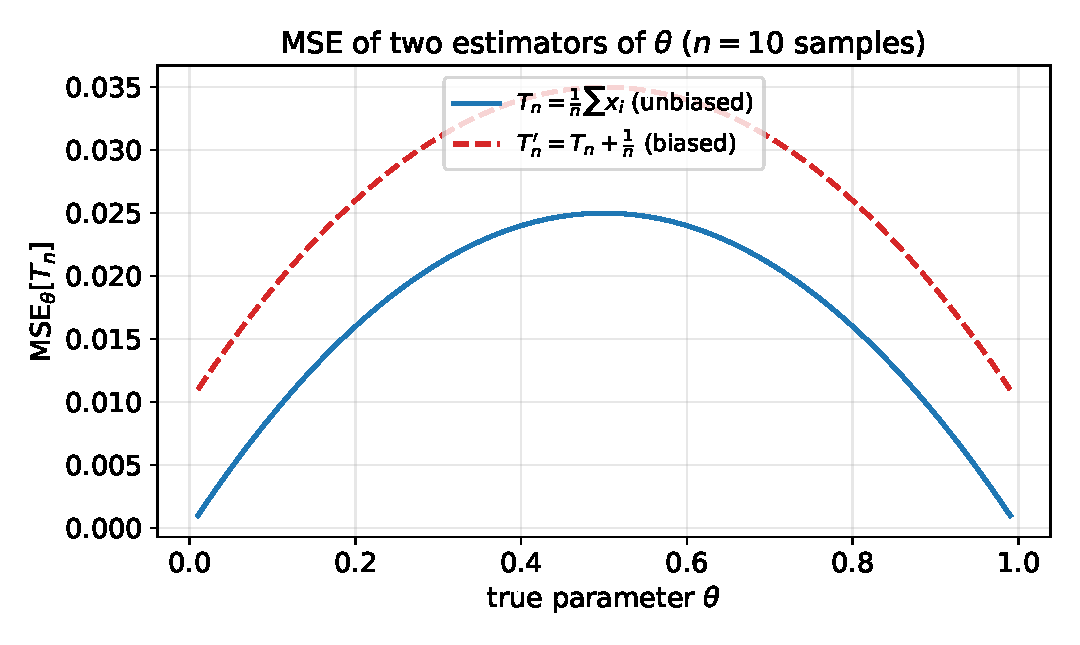
\includegraphics[width=0.62\linewidth]{mse_decomposition}
  \end{center}
  \textbf{Reading the plot.} The dashed (biased) curve sits slightly above
  the solid (unbiased) curve everywhere -- a small, constant MSE penalty
  from the bias term that does not depend on $\theta$. Neither estimator
  ``wins'' by an overwhelming margin here, illustrating that comparing
  estimators can be subtle.
\end{frame}

\begin{frame}{Bias--Variance--MSE Breakdown at $\theta=0.5$}
  \begin{center}
    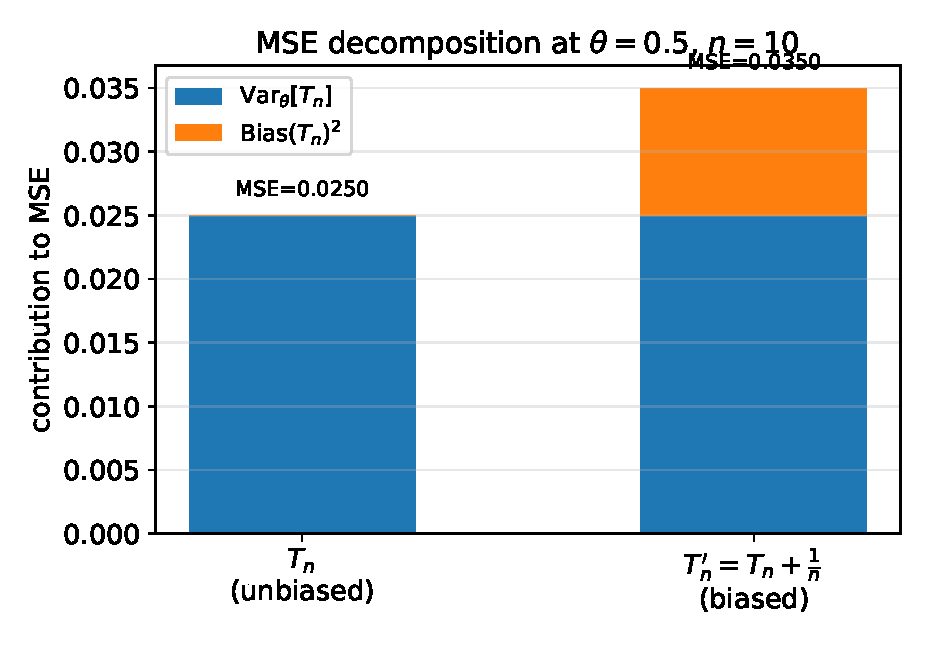
\includegraphics[width=0.58\linewidth]{bias_variance_bars}
  \end{center}
  \textbf{Reading the plot.} Each bar stacks $\mathbf{Var}_\theta[T_n]$
  (blue) below $\mathrm{Bias}(T_n)^2$ (orange); the bar's total height is
  $\mathrm{MSE}_\theta[T_n]$. Here both estimators have identical variance
  ($\theta(1-\theta)/n$), so all the difference in total MSE comes from the
  bias term of $T_n'$.
\end{frame}

\begin{frame}{Definition 2.3.10: Estimator Domination}
  Now that we have a way to compare estimators quantitatively, we can ask:
  is there always a single best choice that beats every other estimator?

  \begin{block}{Definition 2.3.10 (Estimator domination)}
    An estimator $T$ is said to \emph{dominate} another estimator $T'$ if,
    for all choices of parameter $\theta \in \Theta$,
    \[
      \mathrm{MSE}_\theta[T] \;\leq\; \mathrm{MSE}_\theta[T'].
    \]
  \end{block}
  \textbf{Plain English.} $T$ dominates $T'$ if $T$ is never worse, in
  expected squared error, no matter what the true (unknown) $\theta$
  happens to be. This gives only a \emph{partial ordering} -- two
  estimators might each be better than the other for different ranges of
  $\theta$, as in the plot on the previous slide, where the curves nearly
  overlap and neither strictly dominates.

  This raises a natural question: is there a lower bound on how small the
  MSE of an unbiased estimator can possibly be? This motivates studying the
  \emph{score} of a distribution, which underlies the Cram\'er--Rao Bound.
\end{frame}

\begin{frame}{Definition 2.3.11: The Score}
  \begin{block}{Definition 2.3.11 (Score)}
    Given a random variable $X \sim p_X(x;\theta)$ with distribution
    parameterized by $\theta$, the \emph{score} $V$ of $X$ is the random
    variable
    \[
      V \;=\; \nabla_\theta \ln p_X(X;\theta).
    \]
    For a family of random variables $X_1,\dots,X_n \sim
    p_{X_1,\dots,X_n}(x_1,\dots,x_n;\theta)$, the \emph{$n$-sample score}
    $V_n$ is defined analogously using the joint distribution:
    \[
      V_n \;=\; \nabla_\theta \ln p_{X_1,\dots,X_n}(X_1,\dots,X_n;\theta).
    \]
  \end{block}
  \textbf{Plain English.} The score is the gradient (slope) of the
  log-likelihood with respect to $\theta$, evaluated at the (random) data
  itself. It measures \emph{how sensitive} the log-likelihood is to small
  changes in $\theta$ -- and recall that setting this very quantity to zero
  is exactly how we found the MLE.

  One can show that the expected value of the score is zero,
  $\mathbb{E}_\theta[V]=0$, and consequently
  \[
    \mathbf{Var}_\theta[V] \;=\; \mathbb{E}_\theta[V^2].
  \]
  \textbf{Plain English.} Because the score averages to zero, its variance
  is simply the average of its square -- this quantity is called the
  \emph{Fisher information}, and it will be used (beyond what is covered
  in this deck) to bound how good \emph{any} unbiased estimator can be.
\end{frame}

% =============================================================================
\section{Worked Python Examples}
% =============================================================================

\begin{frame}[fragile]{Python: Maximum Likelihood Estimation for a Bernoulli Sample}
  We compute $\widehat{\theta}_{ML} = \frac{1}{n}\sum_i x_i$ directly from a
  small concrete sample, and plot the log-likelihood to confirm the MLE sits
  exactly at its peak.
  \begin{lstlisting}[style=pythonstyle]
import numpy as np

# A concrete coin-flip sample: 1 = heads (sun rose), 0 = tails
x = np.array([1, 0, 1, 1, 0, 1, 1, 1])
n, s = len(x), x.sum()          # n = 8 flips, s = 6 heads

theta_hat_ml = s / n
print(f"MLE estimate theta_hat_ML = {theta_hat_ml:.3f}")
# -> MLE estimate theta_hat_ML = 0.750

# Log-likelihood as a function of theta, for sanity-checking the MLE
def log_likelihood(theta, s, n):
    return s * np.log(theta) + (n - s) * np.log(1 - theta)

thetas = np.linspace(0.01, 0.99, 9901)
theta_argmax = thetas[np.argmax(log_likelihood(thetas, s, n))]
print(f"Numerically maximized theta = {theta_argmax:.3f}")
# -> Numerically maximized theta = 0.750  (matches closed form s/n)
  \end{lstlisting}
\end{frame}

\begin{frame}{The Log-Likelihood Curve, and its Maximum}
  \begin{center}
    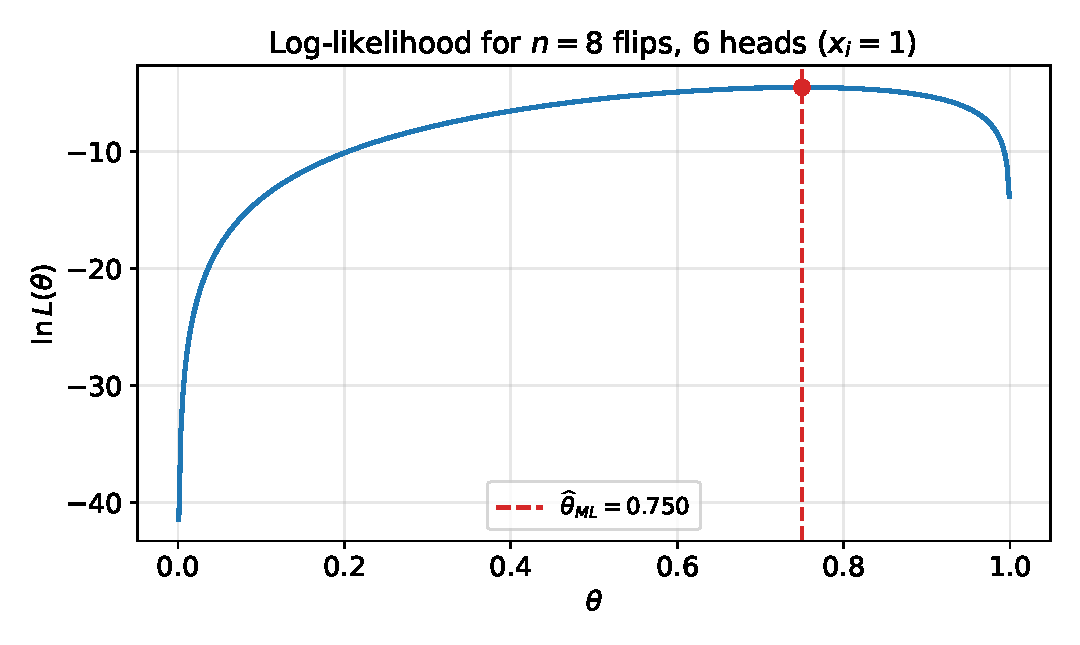
\includegraphics[width=0.62\linewidth]{loglikelihood_bernoulli}
  \end{center}
  \textbf{Reading the plot.} With $n=8$ flips and $s=6$ heads, $\ln
  L(\theta)$ is concave and peaks exactly at $\widehat{\theta}_{ML}=6/8=0.75$
  (red dashed line and dot) -- confirming the closed-form MLE derived by
  setting $\nabla_\theta \ln L(\theta)=0$.
\end{frame}

\begin{frame}[fragile]{Python: Consistency -- MLE Converges as $n$ Grows}
  We simulate a long Bernoulli($\theta=0.7$) sequence and track the running
  MLE estimate $\widehat{\theta}_{ML}(n)$ to see convergence in probability
  in action.
  \begin{lstlisting}[style=pythonstyle]
import numpy as np
rng = np.random.default_rng(42)

theta_true = 0.7
n_max = 500
x = (rng.random(n_max) < theta_true).astype(float)

running_mean = np.cumsum(x) / np.arange(1, n_max + 1)
print("Estimate after n=10  flips:", round(running_mean[9], 3))
print("Estimate after n=100 flips:", round(running_mean[99], 3))
print("Estimate after n=500 flips:", round(running_mean[-1], 3))
# -> Estimate after n=10  flips: 0.800   (noisy -- far from 0.7)
# -> Estimate after n=100 flips: 0.700   (much closer)
# -> Estimate after n=500 flips: 0.702   (very close to true theta)
  \end{lstlisting}
  As $n$ grows, $\widehat{\theta}_{ML}(n)$ settles down near the true
  $\theta=0.7$, illustrating $T_n \xrightarrow{P} \theta$ (Definition 2.3.4).
\end{frame}

\begin{frame}{Visualizing Consistency}
  \begin{center}
    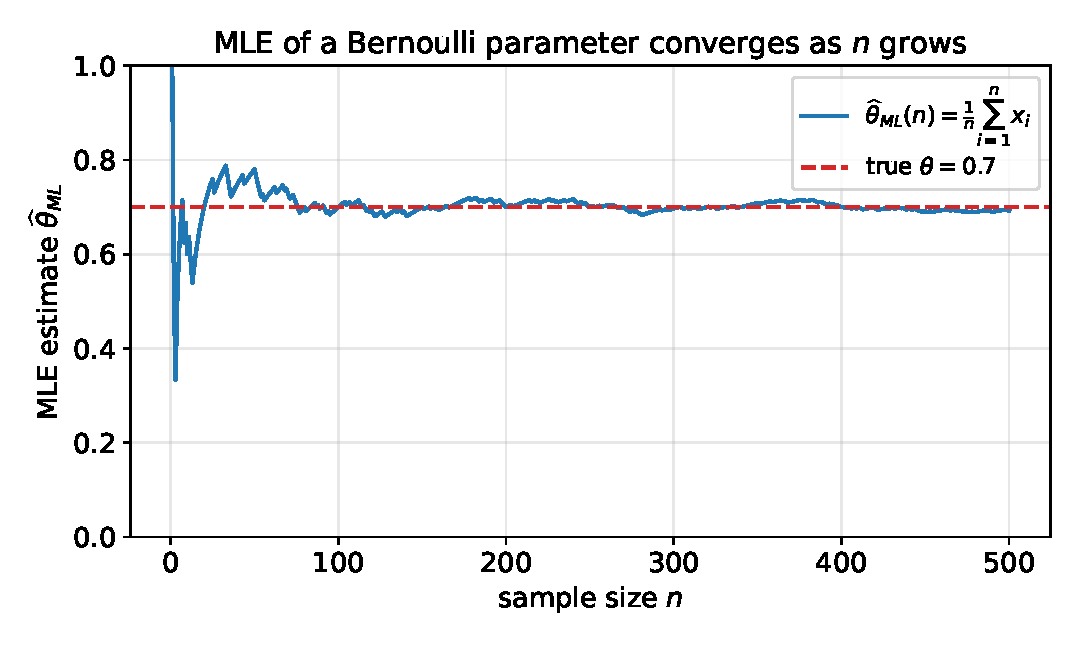
\includegraphics[width=0.62\linewidth]{mle_convergence}
  \end{center}
  \textbf{Reading the plot.} The blue curve is the running MLE estimate
  $\widehat{\theta}_{ML}(n)$ from the code on the previous slide; the red
  dashed line is the true $\theta=0.7$. Early on (small $n$) the estimate is
  noisy and can be far off, but it settles down and converges to the true
  value as $n$ grows -- exactly the behavior Definition 2.3.4 formalizes.
\end{frame}

\begin{frame}[fragile]{Python: Bias and MSE via Monte Carlo Simulation}
  We empirically verify Theorem 2.3.9 ($\mathrm{MSE} = \mathbf{Var} +
  \mathrm{Bias}^2$) for the biased estimator $T_n' = T_n + \frac{1}{n}$ of
  Example 2.3.6, by simulating many independent experiments.
  \begin{lstlisting}[style=pythonstyle]
import numpy as np
rng = np.random.default_rng(0)

theta_true, n, n_trials = 0.5, 10, 200_000

# Simulate n_trials independent experiments, each with n Bernoulli flips
X = (rng.random((n_trials, n)) < theta_true).astype(float)
T  = X.mean(axis=1)          # unbiased estimator T_n
Tp = T + 1.0 / n              # biased estimator T_n' = T_n + 1/n

bias_T,  bias_Tp  = T.mean()-theta_true, Tp.mean()-theta_true
mse_T,   mse_Tp   = ((T-theta_true)**2).mean(), ((Tp-theta_true)**2).mean()
var_T,   var_Tp   = T.var(),  Tp.var()

print(f"T_n:  bias={bias_T:+.4f}  var={var_T:.5f}  MSE={mse_T:.5f}  (Var+Bias^2={var_T+bias_T**2:.5f})")
print(f"T_n': bias={bias_Tp:+.4f}  var={var_Tp:.5f}  MSE={mse_Tp:.5f}  (Var+Bias^2={var_Tp+bias_Tp**2:.5f})")
# -> T_n:  bias~+0.0000  var~0.02500  MSE~0.02500  (Var+Bias^2 ~ 0.02500)
# -> T_n': bias~+0.1000  var~0.02500  MSE~0.03500  (Var+Bias^2 ~ 0.03500)
  \end{lstlisting}
  The empirical MSE matches $\mathbf{Var}+\mathrm{Bias}^2$ to simulation
  precision for both estimators, confirming Theorem 2.3.9 numerically.
\end{frame}

% =============================================================================
\section{Summary}
% =============================================================================

\begin{frame}{Summary: Section 2.3}
  \begin{itemize}
    \item \textbf{Sunrise problem (2.3.1):} naive frequency estimation
      assigns probability $0$ to never-observed events -- an absurd,
      overconfident conclusion that motivates better estimators.
    \item \textbf{Maximum likelihood (2.3.2):} $\widehat{\theta}_{ML}$
      maximizes $L(\theta)=\prod_i p_X(x_i;\theta)$; for Bernoulli data,
      $\widehat{\theta}_{ML} = \frac{1}{n}\sum_i x_i$ (the sample mean), but
      it can be overconfident with little data.
    \item \textbf{Reparametrization equivariance (2.3.3):} the MLE commutes
      with any bijective relabeling of the parameter space.
    \item \textbf{Consistency and bias (2.3.4):} $T_n \xrightarrow{P}
      \theta$ (consistency) and $\mathbb{E}_\theta[T_n]=\theta$
      (unbiasedness) are \emph{independent} properties -- neither implies
      the other.
    \item \textbf{MSE (Def.\ 2.3.8--2.3.10):}
      $\mathrm{MSE}_\theta[T_n]=\mathbf{Var}_\theta[T_n]+\mathrm{Bias}(T_n)^2$
      lets us compare estimators quantitatively via \emph{domination}.
    \item \textbf{Score (2.3.11):} $V=\nabla_\theta \ln p_X(X;\theta)$ has
      mean zero and variance $\mathbb{E}_\theta[V^2]$ -- the Fisher
      information, setting the stage for a lower bound on estimator MSE
      (Cram\'er--Rao Bound).
  \end{itemize}
  \vspace{0.3cm}
  \textbf{Next:} the Bayesian approach to estimation (Section 2.4), which
  treats $\theta$ itself as random and updates a full posterior
  distribution over it as evidence arrives.
\end{frame}

\end{document}
